\chapter{\'Areas de mejora}

El proyecto desarrollado es meramente un prototipo de una aplicación.
En casi todas las fases del proyecto hay aspectos que podrían
mejorarse. A continuación, exponemos algunas de ellas:
\begin{itemize} 
\item Por supuesto, implementar los recursos adecuados para que la 
LOPD no sea un obstáculo para la comercialización del proyecto.
\item Usar un acceso a Twitter que nos permita descargar de forma exhaustiva
la información en relación al perfil de referencia de la oferta de trabajo.
\item Implementar una estructura más escalable, en la nube,
para el manejo de un mayor volumen de datos.
\item En la fase de selección de usuarios:
\begin{itemize}
\item Detección del lenguaje: usar corpus etiquetados para entrenar un modelo,
o usar uno más adecuado para el tipo de lenguaje de los usuarios de Twitter 
(tipo {\tt equilid}).
\item Almacenamiento: usar una base de datos SQL para almacenar los resultados 
intermedios en el proceso, en la nube para mejorar la escalabilidad.
\item Tipo de usuario: explorar otras formas de detectar personas, empresas, bots, etc.. 
Sería interesante incluir un código de reconocimiento facial para identificar si en la foto 
del perfil aparece una persona y añadir el resultado al modelo. También refinar los 
criterios del modelo y explorar nuevos criterios.
\item Naturaleza del tuit: mejorar el modelo para conseguir mayor granularidad en
la clasificación y detectar distintas especialidades dentro del perfil de referencia.
\end{itemize} 
\item En la fase de ordenación de usuarios: explotar más profundamente la información
del grafo, añadiendo características a los nodos, y usar técnicas de detección de comunidades
también para detectar especialidades.
\item En la fase de visualización, adaptar la visualización a un entorno productivo,
quizá incluyendo visualización a través de una página web.
\item Extender la funcionalidad incluida en el proyecto: quizá una monitorización
continua de las publicaciones en Twitter sobre contenidos relacionados con los perfiles de 
referencia para detectar nuevos usuarios relacionados, e ir aumentando el universo de los 
potenciales candidatos (para un servicio continuado a clientes).
\item Añadir otras características a la clasificación final de los candidatos: por ejemplo,
investigar a partir del nombre de usuario de Twitter si dicho usuario tiene un repositorio en 
Github o un usuario activo en StackOverflow para reforzar la relevancia de su perfil.
\end{itemize} 

\section{Mejoras en el algoritmo de clasificación del contenido del tuit}
\label{sect:mejoras_alg_clasificacion_tuit}
En esta sección explicaremos cómo hemos comenzado a trabajar en la mejora del modelo de clasificación descrito en la sección \ref{sect:construccion_modelo_tuits_relevantes}.
Para ello, hemos hechos pruebas con el mismo modelo usado en esa sección, el Multinomial NB, y con otro modelo de clasificación, un SVM, tratando de mejorar los resultados de dos maneras:
\begin{itemize}
\item buscando los mejores parámetros para optimizar la eficiencia del modelo 
(Hyperparameters Optimization) a través del método {\tt GridSearchCV()} y 
\item cambiando el método de entrenamiento, añadiendo al
método sencillo de separación entre entrenamiento y test (que habíamos establecido en $70/30$), 
un algoritmo \lq\lq $K$-fold cross validation\rq\rq, que separa el conjunto de datos en $K$ 
\lq\lq folds\rq\rq o subconjuntos de igual tamaño y cada \lq\lq fold\rq\rq actúa una vez como 
conjunto de test y $K-1$ veces como parte del conjunto de entrenamiento.
\end{itemize}

\subsubsection{Mejorando el modelo {\tt MultinomialNB()} con {\tt GridSearchCV()}
y \lq\lq $K$-fold cross validation\rq\rq}

Con el siguiente código especificamos los parámetros a optimizar, y el método para hacerlo,
un método \lq\lq $K$-fold cross validation\rq\rq (en concreto, con la opción \lq\lq cv = 5\rq\rq):

\medskip

{\tt
\noindent\begin{tabular}{rcl}
parameters &$=$& $\{$'tfidf\_ngram\_range': $[(1,1),(1,2)]$,\\
              &&'tfidf\_use\_idf': $(True, False)$,\\
              &&'tfidf\_sublinear\_tf': $(True, False)$,\\
              &&'tfidf\_min\_df':$(0, 5, 10)$,\\
              &&'tfidf\_max\_df':$(0.95, 0.90, 0.85)$,\\
              &&'clf\_alpha': $(0.001, 0.01, 0.1, 1,10),$\\
			  &&$\}$
\end{tabular}

\noindent text\_cl $=$ Pipeline([('tfidf', TfidfVectorizer()),('clf', MultinomialNB())])

\noindent gs\_clf $=$ GridSearchCV(text\_cl, parameters, cv = 5, scoring='roc\_auc', n\_jobs=-1)

\noindent gs\_clf = gs\_clf.fit(x\_train, y\_train)
    
\noindent\# Aplicando el modelo en la base de test

\noindent gs\_pred = gs\_clf.predict(x\_test)

}


La última línea es la aplicación del modelo al conjunto de test (el $30$\% de los tuits), 
y obtenemos estos resultados:

\begin{center}
\begin{tabular}{ccc}

\begin{tabular}{r|cc}
\multicolumn{3}{c}{\bf Matriz} \\
\multicolumn{3}{c}{\bf de confusión} \\
\hline
\hline
     &$1$&$0$\\
\hline
$1$&$524$&$4$\\
\hline
$0$&$30$&$42$\\
\hline
\end{tabular}

&$$\hspace{2cm}

&\begin{tabular}{r|cccc}
\multicolumn{5}{c}{\bf Métricas de clasificación} \\
\hline
\hline
&Precisión &Recall&F1-score&Support\\
\hline
$0$&$0.95$&$0.99$&$0.97$&$528$\\
\hline
$1$&$0.91$&$0.58$&$0.71$&$72$\\
\hline\hline
Avg/total&$0.94$&$0.94$&$0.94$&$600$\\
\hline
\end{tabular}

\end{tabular}
\end{center}

Respecto a la curva ROC, hemos obtenido
una exactitud (\lq\lq accuracy\rq\rq)
de $0.910208859428$, y la siguiente curva ROC:

\myfigure{
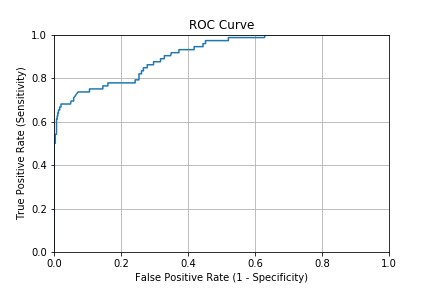
\includegraphics[width=0.7\textwidth]{second_ROC_curve}
\figcaption{Curva ROC de la primera mejora del modelo de clasificación de textos según su relevancia, {\tt MultinomialNB()}.}
\label{fig:second_ROC_curve} 
}


\subsubsection{Cambiamos el modelo a {\tt SVM} con {\tt GridSearchCV()},
también con \lq\lq $K$-fold cross validation\rq\rq}
El código para entrenar este modelo es muy similar al del ejemplo anterior,
y de nuevo tenemos unos parámetros que indican cuáles vamos a optimizar, y una opción
(\lq\lq cv=5\rq\rq) para incluir el algoritmo del \lq\lq $K$-fold cross validation\rq\rq:

\medskip

{\tt
\noindent\begin{tabular}{rcl}
parameters &$=$& $\{$'tfidf\_ngram\_range': $[(1,1),(1,2)]$,\\
              &&'tfidf\_use\_idf': $(True, False)$,\\
              &&'tfidf\_sublinear\_tf': $(True, False)$,\\
              &&'tfidf\_min\_df':$(0, 5, 10)$,\\
              &&'tfidf\_max\_df':$(0.95, 0.90, 0.85)$,\\
              &&'clf\_C': $(1, 10, 100, 1000)$,\\
              &&'clf\_tol':$(0.001, 0.01, 0.1)$,\\
			  &&$\}$
\end{tabular}

\noindent text\_cl $=$ Pipeline([('tfidf', TfidfVectorizer()),
					('clf', LinearSVC())])



\noindent gs\_clf $=$ GridSearchCV(text\_cl, parameters, cv = 5, scoring='roc\_auc', n\_jobs=-1)

\noindent gs\_clf = gs\_clf.fit(x\_train, y\_train)
    
\noindent\# Aplicando el modelo en la base de test

\noindent gs\_pred = gs\_clf.predict(x\_test)

}

A partir de la última línea, la aplicación del modelo al conjunto de test, obtenemos estos resultados:

\begin{center}
\begin{tabular}{ccc}

\begin{tabular}{r|cc}
\multicolumn{3}{c}{\bf Matriz} \\
\multicolumn{3}{c}{\bf de confusión} \\
\hline
\hline
     &$1$&$0$\\
\hline
$1$&$521$&$7$\\
\hline
$0$&$26$&$46$\\
\hline
\end{tabular}

&$$\hspace{2cm}

&\begin{tabular}{r|cccc}
\multicolumn{5}{c}{\bf Métricas de clasificación} \\
\hline
\hline
&Precisión &Recall&F1-score&Support\\
\hline
$0$&$0.95$&$0.99$&$0.97$&$528$\\
\hline
$1$&$0.87$&$0.64$&$0.74$&$72$\\
\hline\hline
Avg/total&$0.94$&$0.94$&$0.94$&$600$\\
\hline
\end{tabular}

\end{tabular}
\end{center}

En la curva ROC para este modelo, hemos obtenido
una exactitud (\lq\lq accuracy\rq\rq)
de $0.952033354377$, y la siguiente gráfica:

\myfigure{
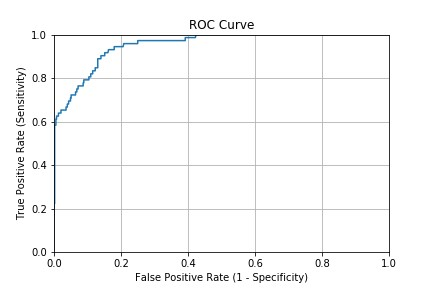
\includegraphics[width=0.7\textwidth]{third_ROC_curve}
\figcaption{Curva ROC del modelo {\tt LinearSVC()}.}
\label{fig:third_ROC_curve} 
}

\subsubsection{Conclusión}

Los dos modelos han resultado producir una \lq\lq accuracy\rq\rq y métricas muy parecidas. El modelo SVM tal vez aventaje ligeramente al Naïve Bayes. Sin embargo, el Naïve Bayes tiene un procesamiento más rápido y sencillo. Por eso creemos que será necesario incluir los dos modelos en el proyecto para llegar a una conclusión, pero si en el futuro es necesario tener velocidad, usaríamos el Naïve Bayes.
